%% LyX 1.3 created this file.  For more info, see http://www.lyx.org/.
%% Do not edit unless you really know what you are doing.
\documentclass[english,dvips]{cfdsc}
\usepackage{pslatex}
\usepackage[T1]{fontenc}
\usepackage[latin1]{inputenc}
\usepackage{geometry}
\geometry{verbose,letterpaper}
\pagestyle{empty}
\usepackage{subfigure}
\usepackage{graphicx}

\makeatletter

%%%%%%%%%%%%%%%%%%%%%%%%%%%%%% LyX specific LaTeX commands.
%% Bold symbol macro for standard LaTeX users
\providecommand{\boldsymbol}[1]{\mbox{\boldmath $#1$}}


%%%%%%%%%%%%%%%%%%%%%%%%%%%%%% User specified LaTeX commands.
\usepackage{url}
\renewcommand{\textfraction}{0}
\renewcommand{\floatpagefraction}{1.}
\renewcommand{\topfraction}{1.}
\renewcommand{\dblfloatpagefraction}{1.}
\renewcommand{\dbltopfraction}{1.}

\usepackage{babel}
\makeatother
\begin{document}

\title{Interoperable Software Components for CFD}


\author{Carl Ollivier-Gooch\inst{1} \and Kyle Chand\inst{2} \and Tamara
Dahlgren\inst{2} \and Lori Freitag Diachin\inst{2} \and Brian
Fix \inst{3} \and Jason Kraftcheck\inst{4} \and Xiaolin Li\inst{3}
\and E. Seegyoung Seol\inst{5} \and Mark S. Shephard\inst{5} \and
Timothy Tautges\inst{4} \and Harold Trease\inst{6} }


\institute{Advanced Numerical Simulation Laboratory, University of British Columbia
\and Center for Applied Scientific Computing, Lawrence Livermore
National Laboratory \and Dept. of Applied Mathematics and Statistics,
SUNY Stonybrook \and Parallel Computing Sciences, Sandia National
Laboratories \and Scientific Computation Research Center, Rensselaer
Polytechnic Institute \and Pacific Northwest National Laboratory}


\email{cfog@mech.ubc.ca}

\maketitle

\section{Introduction}

Creating automated, reliable and flexible CFD codes requires the use
of advanced techniques in a variety of areas. For example, automatic
mesh generation and adaptation contribute significantly to simulation
automation and reliability, while robust discretization schemes and
error control are central components to solution reliability. As new
and better techniques for discretization, flux calculation, turbulence
modeling, and multi-disciplinary coupling are developed, existing
modules in CFD software must be enhanced or replaced to take advantage
of these new tools. Traditionally, four approaches have been used
to provide tools and technologies to CFD code developers: 

\begin{enumerate}
\item Complete \emph{simulation codes} that support the integration of specific
user-defined modules (e.g., Fluent~\cite{fluent:http}) are most
useful for enhancing existing physics capabilities of the simulation
code.
\item \emph{Simulation} \emph{frameworks} that support the overall development
process (e.g. FEMLab~\cite{femlab}) can be both powerful and flexible,
but are aimed primarily at development of new simulation codes, not
enhancement of existing codes.
\item \emph{Libraries} that support specific aspects of the simulation process
(e.g., LAPACK~\cite{lapack} or PETSc~\cite{petsc} for numerical
linear algebra) typically provide important supporting infrastructure
for a simulation, with the drawback that different libraries express
essentially the same functionality differently at the programming
level.
\item \emph{Components} are software objects that encapsulate specific functionalities
using a clearly-defined interface. Typically, each interface is supported
by multiple implementations which allows code developers to easily
experiment with different approaches. 
\end{enumerate}
While each of these approaches is useful under some circumstances,
this paper will focus on the component approach. The primary difference
between a component and a library --- and the primary advantage of
using components --- is that a component has a fixed API, and so applications
can use components interchangeably, as opposed to a library, where
changing from one to another requires (perhaps significant) re-programming
effort. Because components have a specifically prescribed interface
and behavior, application-component and component-component interactions
are much simpler than in the other cases listed above --- replacing
one component with another requires no re-writing of existing code.
The use of components is ideal in the case where there is already
a substantial investment in the simulation code and the developers
are interested in incorporating advanced functionality or experimenting
with several different, related approaches. 

This paper introduces the work of the Terascale Simulation Tools and
Technologies (TSTT) consortium to develop components for mesh, geometry,
and field functionality, including general relationships between them.
In addition to defining interfaces for these components, members of
the consortium are adding support for these interfaces to their existing
tools. We discuss the component paradigm and its application to CFD
simulations in more detail in Section~\ref{sec:The-Component-Paradigm}. 

Essential to the development of any software component is a clear
definition of an abstract data model describing the type of data on
which the component will operate; the TSTT data model is described
in Section~\ref{sec:TSTT-Data-Model}. The scope of each of the interfaces
--- mesh, geometry, fields, and relationships --- and a summary of
the functionality of each is given in Section~\ref{sec:The-TSTT-Interfaces}.


\section{The Component Paradigm\label{sec:The-Component-Paradigm}}

All CFD application codes, by necessity, store and manipulate both
mesh data and solution data discretized on that mesh. Beyond this
fundamental similarity, however, lie a dizzying array of ways to represent
and retrieve data, each with its advantages for particular scenarios.
However, these variations make it essentially impossible to employ
software modules written by other developers because of data structure
incompatibilities, as suggested in Figure~\ref{fig:current-scenario}.%
\begin{figure}
\begin{center}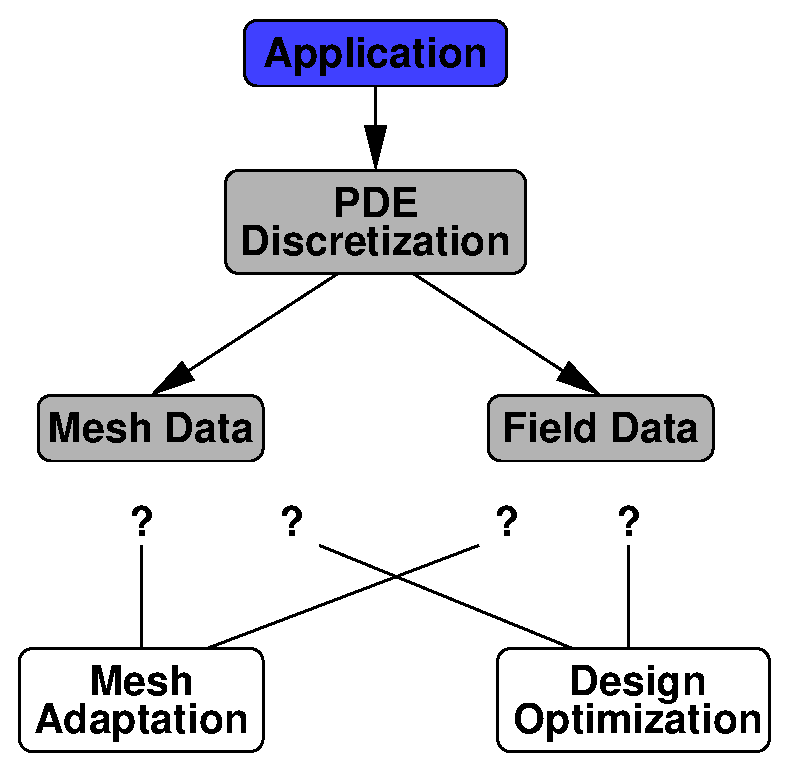
\includegraphics[%
  width=1.0\columnwidth]{non-component.eps}\end{center}


\caption{Current typical scenario for interfacing existing code with external
services.\label{fig:current-scenario}}
\end{figure}


In the component programming paradigm, the data model and application
programming interface (API) for a particular set of functionality
is standardized as a \emph{component}. In this way, tools like mesh
adaptation can exploit the standard functionality of a mesh interface
without needing explicit information about how that functionality
is implemented. If the code from the previous example were to provide
access to its data structures through a component API, adding additional
functionality would be trivial, since existing services based on the
API could be used for the effort of compiling and linking them, as
shown in Figure~\ref{fig:wrapper}.%
\begin{figure}
\begin{center}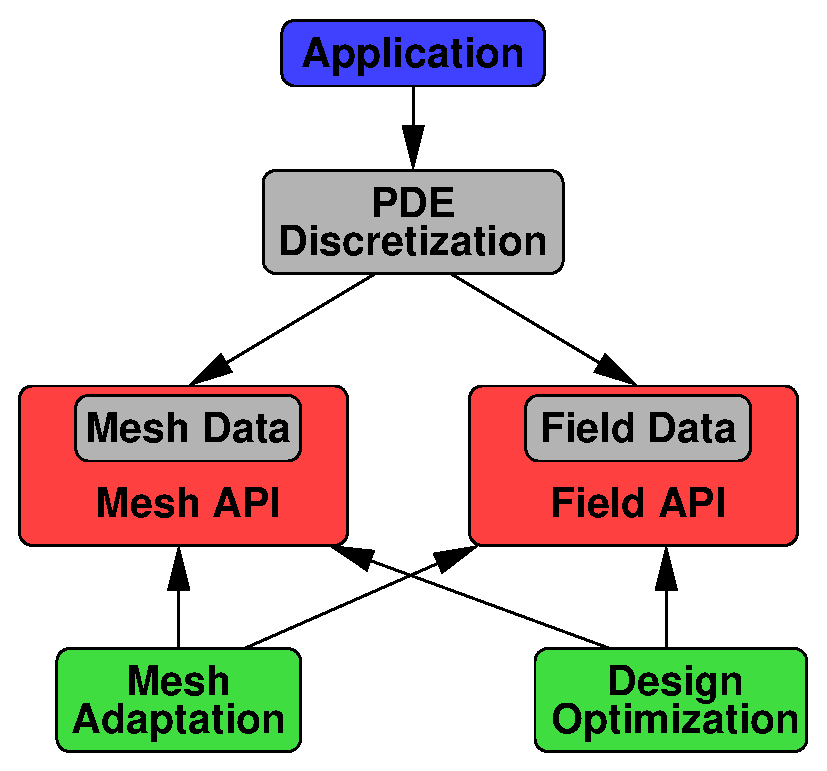
\includegraphics[%
  width=1.0\columnwidth]{wrapper.eps}\end{center}


\caption{Wrapping existing data in a component API supports use of off-the-shelf
services written to use that API.\label{fig:wrapper}}
\end{figure}
 

The component paradigm supports both horizontal and vertical interoperability.
Horizontal interoperability implies that multiple services exist that
use the same interface to perform the same task, and an application
can choose whichever one best suits its purposes. For instance, two
interfaces may be available to query CAD-based geometric data, but
one interface might support a CAD file format that the other doesn't.
Vertical interoperability implies that services at different levels
of complexity can be combined to create a high-level application.
For instance, implementations of basic geometry query and mesh query
and modification components could be combined with services that perform
vertex insertion and topology change to create a mesh generation application.

Overall, we envision at least four possible usage modes for our mesh,
geometry, and field component interfaces.%
\begin{figure*}
\noindent \subfigure[Component interface wrapper for an existing implementation.]{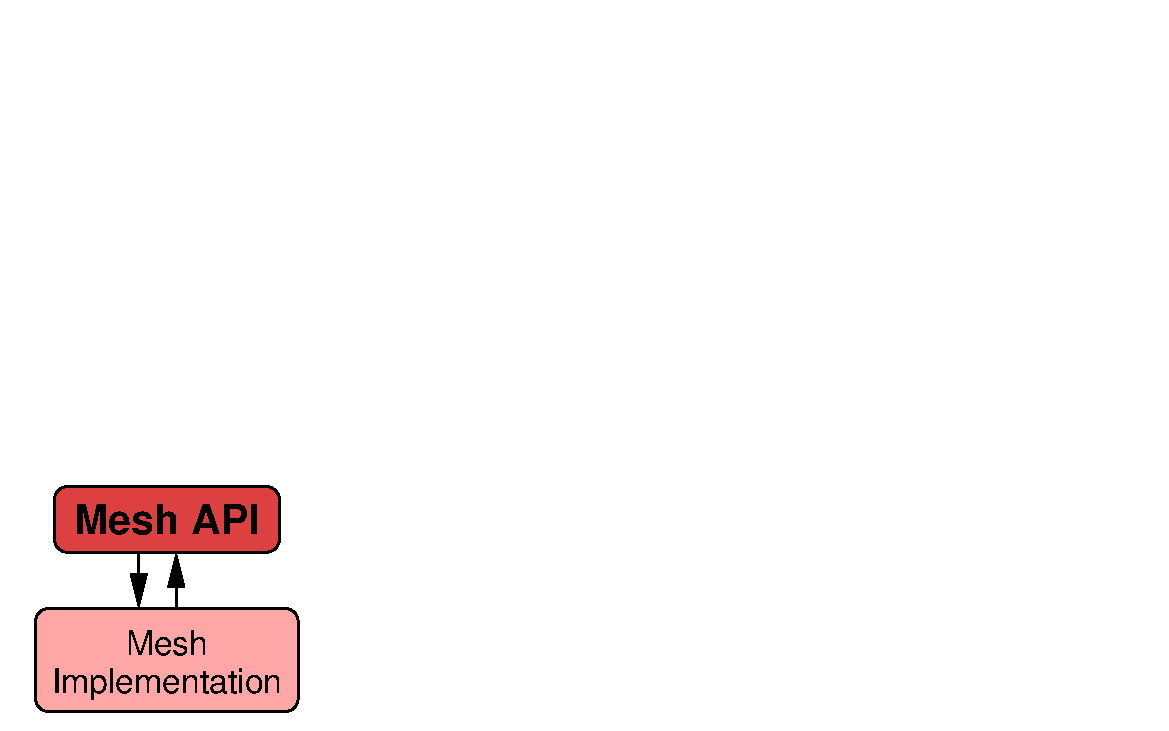
\includegraphics[%
  width=1.0\columnwidth]{implementation.eps}}\hfill{}\subfigure[Service built on component API's.]{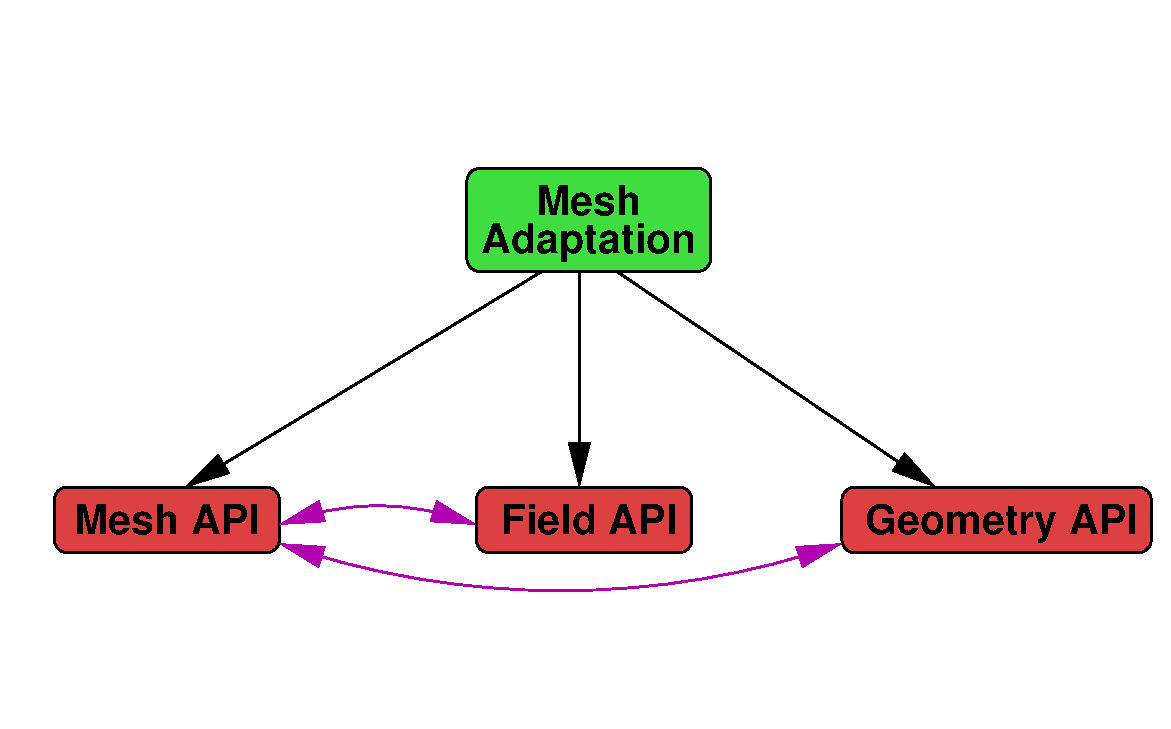
\includegraphics[%
  width=1.0\columnwidth]{service.eps}}\\
\subfigure[Application using builtin API for internal data and external implementations of other components.]{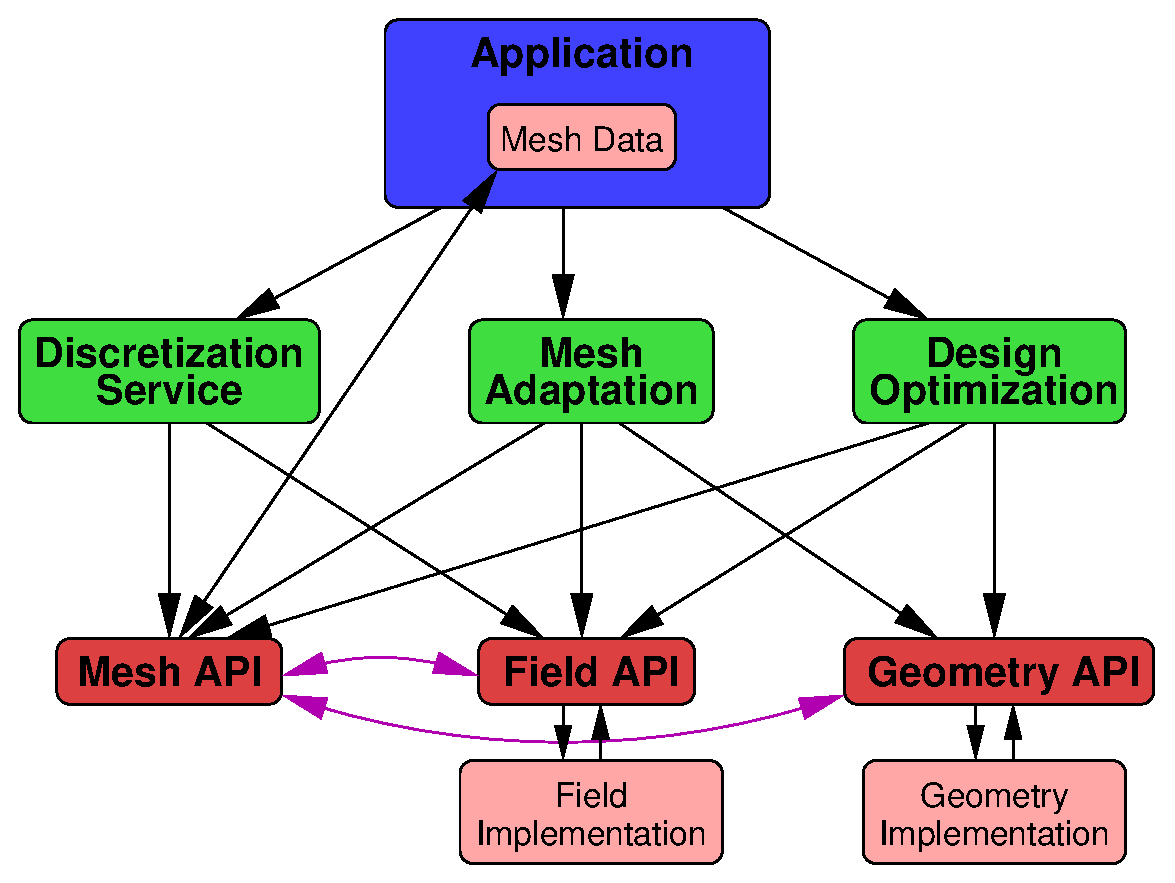
\includegraphics[%
  width=1.0\columnwidth]{app-serv.eps}}\hfill{}\subfigure[Application constructed from high-level services using external implementations for all low-level components.]{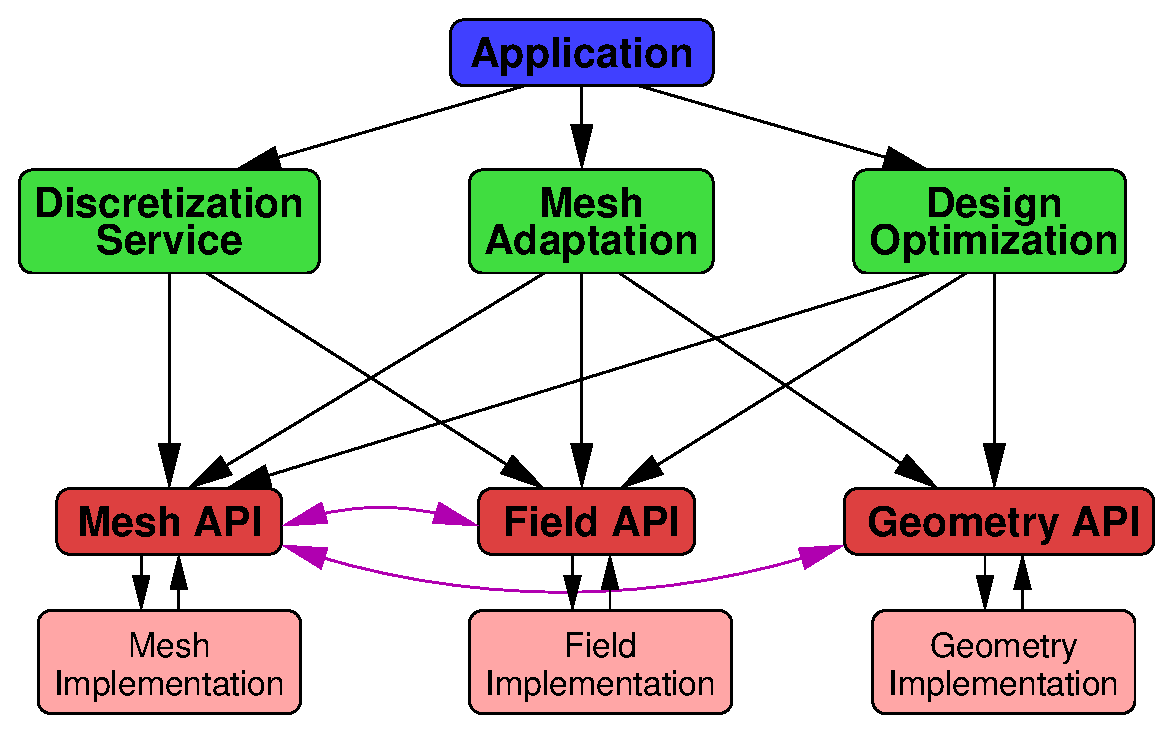
\includegraphics[%
  width=1.0\columnwidth]{app-serv-impl.eps}}


\caption{Possible usage modes for mesh, geometry, and field components.\label{fig:Possible-usage-modes}}
\end{figure*}


\begin{enumerate}
\item At the lowest level, we expect to see implementations of the basic
interfaces, typically built on existing software infrastructure (mesh
databases, geometry modelers, etc; see Figure~\ref{fig:Possible-usage-modes}a).
\item Algorithms for common tasks, including mesh manipulation and discretization
tasks, can be written as services that use the TSTT interface, and
are then interoperable between implementations of the interface (Figure~\ref{fig:Possible-usage-modes}b).
\item Applications that already have infrastructure can take advantage of
TSTT-based services by providing access to their internal data structures
through TSTT interfaces (Figure~\ref{fig:Possible-usage-modes}c).
\item Applications can be largely assembled from existing implementations
and services, in much the same way that simulation frameworks are
currently used (Figure~\ref{fig:Possible-usage-modes}d).
\end{enumerate}

\section{TSTT Data Model\label{sec:TSTT-Data-Model}}

The TSTT data model partitions the data required by a simulation into
three \textit{core data types}: the geometric data, the mesh data,
and the field data. Interfaces to the data represented by these abstractions
channel the flow of information throughout the simulation. For example,
TSTT adaptive mesh refinement services access solution information
for error estimation via the field interface; modify the mesh using
the mesh interface; and query the geometry interface when creating
mesh entities on domain boundaries. These core data types are associated
with each other through \textit{data relation managers}. The data
relation managers control the relationships among two or more of the
core data types, resolve cross references between entities in different
groups, and can provide additional functionality that depends on multiple
core data types. 

A key aspect of the TSTT approach is that we do not enforce any particular
data structure or implementation with our interfaces, requiring only
that certain questions about the geometry, mesh, or field data can
be answered through calls to the interface. To encourage adoption
of the interface, we aim to create a small set of interfaces that
existing mesh and geometry packages can support. The latter point
is critical: hundreds of person-years have been invested in the development
of a wide variety of geometry, mesh generation and mesh management
toolkits. These software packages will not be rewritten from scratch
to conform to a common API; rather the API must be data structure
neutral and allow for a broad range of underlying mesh, geometry,
and field representations. However, only a small set of functionalities
can be covered by a 'core' set of interface functions. To increase
the functionality of the TSTT interface, we define additional, optional,
interfaces for which we will provide reference implementations based
on the core interface methods. Developers can incrementally adopt
the interface by implementing the optional functions on their own
mesh database as needed.

The TSTT data models for mesh, geometry and fields all make use of
the concepts of \textit{entities}, \textit{entity sets}, and \textit{tags},
and we describe these now in some detail.


\subsection{Entities}

TSTT \textit{entities} are used to represent atomic pieces of information
such as a vertices in a mesh or edges in a geometric model. To allow
the interface to remain data structure neutral, entities (as well
as entity sets and tags) are uniquely represented by opaque handles.
Unless entities are added or removed, these handles must be invariant
through different calls to the interface in the lifetime of the TSTT
interface, in the sense that a given entity will always have the same
handle. Access to entities and their data is provided through the
mesh, geometry or field interfaces, which we describe in detail in
the sections that follow.

Entity adjacency relationships define how the entities connect to
each other and both first-order and second-order adjacencies are supported
for the mesh and geometry interfaces. 

\begin{itemize}
\item \textit{First-order adjacencies}: For an entity of dimension $d$,
first-order adjacencies return all of the entities of dimension $q$,
which are either on the closure of the entity ($d>q$, downward adjacency),
or which it is on the closure of ($d<q$, upward adjacency).
\item \textit{Second-order adjacencies}: Many applications require not only
information about first-order adjacencies, but also about the next
level of neighbors. Although such information can always be determined
from the appropriate first-order adjacencies, their application is
common enough that supporting a second-order adjacency function is
useful. A second-order adjacency determines the set of topological
entities of a given type adjacent to entities that share common boundary
entities of the specified type. An example would be the set of regions
that share a bounding edge with the given region. 
\end{itemize}

\subsection{Entity Sets}

A TSTT \textit{entity set} is an arbitrary collection of TSTT entities
that have uniquely defined entity handles. Each entity set may be
an unordered set or it may be a (possibly non-unique) ordered list
of entities. When a TSTT mesh, geometry or field object is first created
in a simulation, a \textit{root set} is created and can be populated
by using the load functionality of the object.

Two primary relationships among entity sets are supported:

\begin{itemize}
\item Entity sets may \textit{contain} one or more entity sets. An entity
set contained in another may be either a subset or an element of that
entity set. The choice between these two interpretations is left to
the application; TSTT supports both interpretations. If entity set
A is contained in entity set B, a request for the contents of B will
include the entities in A and the entities in sets contained in A
if the application requests the contents recursively. We note that
the \textit{root set} cannot be contained in another entity set.
\item \textit{Parent/child relationships} between entity sets are used to
represent relations between sets, much like directed edges connecting
nodes in a graph. This relationship can be used to indicate that two
meshes have a logical relationship to each other, including multigrid
and adaptive mesh sequences. Because we distinguish between parent
and child links, this is a directed graph. Also, the meaning of cyclic
parent/child relationships is dubious, at best, so graphs must be
acyclic. No other assumptions are made about the graph. 
\end{itemize}
Users are able to query entity sets for their entities and entity
adjacency relationships. Both array- and iterator-based access patterns
are supported. In addition, entity sets also have \char`\"{}set operation\char`\"{}
capabilities; in particular, existing TSTT entities may be added to
or removed from the entity set, and sets may be subtracted, intersected,
or united.


\subsection{Tags}

TSTT \textit{tags} are used as containers for user-defined opaque
data that can be attached to TSTT entities and entity sets. Tags can
be multi-valued which implies that a given tag handle can be associated
with many different entities. In the general case, TSTT tags do not
have a predefined type and allow the user to attach any opaque data
to TSTT entities. To improve ease of use and performance, we support
three specialized tag types: integers, doubles, and entity handles.
Tags have and can return their name (as a string), size, handle and
data. Tag data can be retrieved from TSTT entities by handle in an
agglomerated or individual manner. The TSTT implementation is expected
to allocate the memory as needed to store the tag data.


\section{The TSTT Interfaces\label{sec:The-TSTT-Interfaces}}


\subsection{The Mesh Interface}

\label{sec:mesh}

TSTT \textit{mesh entities} are the fundamental building blocks of
the TSTT mesh interface and correspond to the individual pieces of
the domain decomposition (mesh). Specific examples of mesh entities
include, for example, a hexahedron, tetrahedron, edge, triangle and
vertex. Mesh entities are classified by their entity type (topological
dimension) and entity topology (shape). Allowable mesh entity types
are vertex (0D), edge (1D), face (2D), and region (3D). Allowable
entity topologies are point (0D); line segment (1D); triangle, quadrilateral,
and polygon (2D); and tetrahedron, pyramid, prism, hexahedron, septahedron,
and polyhedron (3D); each of these topologies has a unique entity
type associated with it. Mesh entity geometry and shape information
is associated with the individual mesh entities. For example, the
vertices will have coordinates associated with them. Higher-dimensional
mesh entities can also have shape information associated with them.
For example the coordinates of higher-order finite-element nodes can
be associated with mesh edges, faces, and regions. 

Higher-dimensional entities are defined in terms of the lower-dimensional
entities on their closure (for instance, a triangle could be defined
by a list of edges or by a list of vertices) with shape and orientation
determined using canonical ordering relationships. Because not all
implementations support all possible adjacency relationships, an application
can request an \emph{adjacency table} by using a query through the
interface. The adjacency table reports, for each possible upward and
downward adjacency, whether that adjacency information is always,
sometimes, or never available; and to be available at a cost that
is constant, logarithmic (i.e., tree search), or linear (i.e., search
over all entities) in the size of the mesh. If adjacency information
exists, entities must be able to return information in the canonical
ordering using both individual and agglomerated request mechanisms.

TSTT \textit{mesh entity sets} are extensively used to group mesh
entities in meaningful ways, for example, to represent the set of
all faces classified on a geometric face, or the set of regions in
a partition for parallel computing. For some computational applications,
it is useful for entity sets to comprise a valid computational mesh.
The simplest example of this is a non-overlapping, connected set of
TSTT region entities, such as the structured and unstructured meshes
commonly used in CFD simulations. Collections of entity sets can compose,
for example, overlapping and multi-block meshes. In both of these
examples, supplemental information on the interactions of the mesh
sets will be defined and maintained by the application. Smooth particle
hydrodynamic (SPH) meshes can consist of a collection of TSTT vertices
with no connectivity or adjacency information.

The mesh interface also includes modification operators that change
the geometry and topology. Capabilities include changing vertex coordinates
and adding or deleting entities. No validity checks are provided with
this basic interface so that care must be taken when using these interfaces.
These interfaces are intended to support higher-level functionality
such as mesh quality improvement, adaptive schemes, front tracking
procedures, and basic mesh generation capabilities, all of which would
provide validity checking. Modifiable meshes require interactions
with the underlying geometric model including classifying entities.


\subsection{The Geometry Interface}

The geometry interface provides access to the topology and shape of
a geometric model, including the ability to modify the topology and
shape as required by optimization and moving body problems. The interface
is defined with the intent of supporting both commercial modelers
(which often have an underlying parametric surface representation)
and models constructed from an input mesh (which typically are not
parametric). In the latter case, some algorithm (for example,~\cite{KrOr01,PaOr02,WaKo04})
must be used to combine appropriate mesh entities into geometric entities.

Most geometry queries in mesh-based simulations are requests for information
from a particular geometric entity: a region, a face, an edge, or
a vertex. A few situations, particularly those dealing with evolving
geometry, will have need for the additional topological constructs
of loops and shells (represented in TSTT as sets of faces and edges,
respectively). Typical geometric shape queries can be expressed either
in physical coordinates or in parametric coordinate. The latter are
much more efficient --- as much as two orders of magnitude --- but
are not always available. To maximize efficiency while still providing
general functionality regardless of the underlying shape representation,
the TSTT geometry interface provides both parametric and non-parametric
versions of all shape queries.

The geometric interface functions are grouped by the level of geometric
model information needed to support them and the type of information
they provide.% \cite{TSTT-software}
The base level includes:

\begin{description}
\item [Model~loading.]This includes not only reading the model data, but
also initiating any supporting processes (such as a CAD engine) and
pre-processing the data as required (for example, producing a piecewise
spline surface from mesh data).
\item [Adjacency~queries]for regions, faces, edges, and vertices in the
geometric model.
\item [Iterators]over regions, faces, edges, and vertices.
\item [Geometric~shape~interrogations.]Typical functions include returning
the closest point on a model entity, getting coordinates, normals,
tangents and curvatures, and requesting bounding boxes of entities.
\item [Tag]functionality, to associate user-defined information with entities. 
\end{description}
Other groups of functions increase the functionality and/or the efficiency
of the interface. Functions of this type that have been defined for
the geometry interface include: 

\begin{description}
\item [Geometric~sense~information]indicating how face normals and edge
tangents are oriented. 
\item [Parametric~coordinates]for edges and faces. The functions in this
group include conversion between global and parametric coordinates,
conversion between parametric coordinates of points on the closure
of multiple entities, and the full set of pointwise geometric interrogations
for a point given its parametric coordinates on a particular geometric
entity.
\item [Tolerance~information.]These functions provide access to the geometric
modeling tolerances used by the modeling system in the determination
of how closely adjacent entities must be matched. This information
is essential, for instance, when constructing viscous meshes near
the intersection of two surfaces.
\end{description}
Additional functions of value to specific mesh-based applications
that have not yet been defined include: 

\begin{description}
\item [General~topology.]The functions described above do not directly
support shells and loops, and do not support non-manifold geometries
at all. 
\item [Model~modification,]both topological and geometric.
\end{description}

\subsection{The Field Interface}

The TSTT field interface is intended to provide solution data in a
form that supports queries and other operations by external software.
Two common situations in which fields are a useful construct are multiphysics
analysis, where the solution (or some derived quantity) from one physical
problem provides a boundary condition or forcing function for another;
and the implementation of mesh adaptation services, where solution
fields are used to estimate error and hence the new mesh size and
shape distribution. In each of these cases, the use of a field interface
hides the way that solution data is treated by the underlying implementation,
enabling interchange of physics modules or of adaptation drivers without
changing how data is accessed.

Physical information about the dependent flow variables in a CFD simulation
can be represented by using tensor quantities, including density (rank
0), velocity (rank 1), and viscous stress (rank 2). While physically
these variables are defined at all points in the flow, a field contains
only a discrete representation of the variable, stored as a collection
of discrete values called degrees of freedom. Each field representation
has a method for using \emph{}this discrete data to compute variable
values at all locations; regardless of the underlying discretization
scheme, this conversion from discrete to piecewise continuous data
is primarily a geometric operation. For example, finite element and
discontinuous Galerkin methods use shape functions to compute data
at arbitrary locations, while unstructured finite volume methods use
reconstruction.

A complex simulation process can involve a number of fields defined
over various portions of the domain of the simulation. A single field
can be used by a number of different analysis routines that interact,
and the field may be associated with multiple meshes and have a different
relationship with each one. In addition, different distributions can
be used by a field to discretize its associated tensor. The ability
to have a specific tensor defined over multiple meshes and/or discretized
in terms of multiple distributions is handled by supporting multiple
instances. A field instance has a single set of distributions over
a given mesh. 

The TSTT consortium is currently defining interoperable functions
for field I/O, interrogation, coordinate transforms, and transfer
between field instances. The latter capability is useful, for instance
in projecting a discontinuous stress field onto a set of continuous
shape functions or transferring pressure data from a finite volume
flow solution to a finite element solid mechanics solver. 


\subsection{Relationships Between Data in Different Interfaces}

In addition to functions that operate only on mesh data or only on
geometric, the TSTT interface contains functions to relate mesh, geometry,
and field data. For instance, \emph{classification} of mesh faces
onto faces of a geometric model is accomplished through the relations
interface. In addition to simple set and query functions for one-to-one
and one-to-many relationships, the relations interface contains advanced
functionality to support deduction of relationships among data of
different data. For instance, a mesh file may contain tags that indicate
classification of mesh entities onto a geometric model; the relations
interface essentially prompts the mesh implementation to convert that
tag data into relationships between mesh and geometry entities, which
can then be accessed in a standard way through the relations interface.


\section{Current Status and Future Plans\label{sec:Current-Status}}


\subsection{Implementation of the Interfaces}

The mesh interface definition effort is complete, and several implementations
are also nearly complete, which are built on existing mesh management
toolkits: FMDB (RPI)~\cite{ReSh03}, GRUMMP (UBC)~\cite{GRUMMP:http},
MOAB (SNL)~\cite{moab,moab:http}, NWGrid (PNNL)~\cite{nwgrid:http},
and Overture (LLNL)~\cite{overture:http,overtureTR}. The geometry
interface is essentially complete, and implementation efforts are
underway, based on the CGM (SNL)~\cite{Ta00,Tau01} geometry toolkit.
The field interface definition is not yet complete, and so no implementations
that support it directly exist at present.


\subsection{Services Built on the Interfaces}

Several services have been built on top of the current interfaces.
Strictly speaking, these services are themselves components, with
their own interfaces. Unlike the mesh, geometry, and field interfaces,
which encapsulate data and data access, the services encapsulate \emph{algorithms}.
Because the mesh interface and its implementations are the most mature,
most current services are built on the mesh interface. These include
mesh swapping~\cite{TSTT-swap-tool}, smoothing~\cite{Mesquite03},
and adaptation~\cite{LiSh05}; these services also require at least
some access to mesh geometry information. Other services currently
under development include front-tracking (based on FronTier~\cite{FixGlimm})
and general mesh and geometry access (based on MOAB~\cite{moab,moab:http}
and CGM~\cite{Ta00,Tau01}).


\subsection{Future Plans}

One of the main short-term technical goals of the TSTT consortium
is to complete the definition of the fields interface and implement
it. This will open up a new range of possible services, including
mesh-to-mesh solution transfer, a general AMR service, and discretization
support services. Also planned for the short-term, in conjunction
with applications projects, are a shape optimization service and services
to generate and manipulate meshes in parallel.


\section*{Acknowledgments}

This work was performed under the auspices of the U.S. Department
of Energy by the University of California Lawrence Livermore National
Laboratory under contract No. W-7405-Eng-48 (UCRL-JRNL-213577); the
Canadian Natural Sciences and Engineering Research Council under Special
Research Opportunities Grant SRO-299160; and by Rensselaer Polytechnic
Institute under DOE grant number DE-FC02-01ER25460.

\bibliography{tstt}

\end{document}
